\chapter{Технические методы}
\begin{important}
Не стоит забывать, что следующие методы необходимо использовать, по возможности, совместно друг с другом и с методами, перечисленными в предыдущей главе.
\end{important}
\section{Прокси}

\section{VPN}

\section{SSH-туннели}

\section{Настойка браузера Firefox}
\subsection{Подмена информации, передаваемой браузером}
\begin{important}
Браузер передает огромное количество информации. По отдельности эта информация не представляет никакого интереса, но собранная вместе она может позволить практически со 100\% вероятностью установить вашу личность.
\end{important}
\subsubsection{User-agent}
\subsubsection{Часовой пояс}
\subsubsection{Предпочитаемые языки}
\subsection{Дополнения}
\subsubsection{HTTPS Everywhere}
\textbf{HTTPS Everywhere} --- дополнение для браузеров Firefox и Chrome/Chromium, переадресующее на HTTPS версию сайта, если она доступна. Это позволяет защититься от перехвата передаваемых данных, но не позволяет скрыть сам факт посещения вебсайта. Скачать дополнение можно тут \url{https://eff.org/https-everywhere}.
\subsubsection{BetterPrivacy}
\subsubsection{Ghostery}
\subsubsection{TrackerBlock}
\subsubsection{Beef Taco}
\subsubsection{User Agent Changer}

\section{Анонимные оверлейные сети}
\textbf{Оверлейные сети} --- это такие сети, которые работают поверх другой уже работающей сети.
\subsection{Tor}
\begin{wrapfigure}[9]{r}{0.25\linewidth}

\includegraphics[width=\linewidth]{Tor}
\caption{Логотип Tor}
\end{wrapfigure}
\textbf{Tor} --- анонимная оверлейная сеть, использующая принцип луковой маршрутизации, исходные коды которой распространяются на условиях лицензии BSD\cite{tor_license}.\\
\textbf{Луковая маршрутизация} --- технология анонимного обмена информацией, использующая многократное шифрование и пересылку через цепочки узлов. Каждый луковый маршрутизатор в цепочке удаляет слой шифрования и пересылает сообщение дальше, согласно полученным инструкциям, где все повторится. И так до тех пор, пока сообщение не достигнет адресата. Такое название технология получила из-за сходства данного процесса с очисткой луковицы.\\
\subsubsection{Установка}
Для установки посетите \url{https://torproject.org} или установите пакет с помощью пакетного менеджера вашего дистрибутива.
\subsubsection{Использование}
\subsubsection{Недостатки}
\begin{important}
Не забывайте, что при использовании обычного Интернета через Tor, последняя нода в цепочке (exit-нода) видит трафик нешифрованным.
\end{important}
\subsection{I2P}
\begin{wrapfigure}[6]{r}{0.25\linewidth}

\includegraphics[width=\linewidth]{I2P}
\caption{Логотип I2P}
\end{wrapfigure}
\textbf{I2P} --- анонимная оверлейная сеть, использующая принцип чесночной маршрутизации, исходные коды которой распространяются на условиях нескольких свободных лицензий\cite{i2p_license}. В отличии от Tor, который в первую очередь направлен на доступ к сайтам обычного интернета (хотя в нем и существуют скрытые сервисы, аналогичные ипсайтам в I2P, а в I2P можно получить доступ к внешнему Интернету, используя аутпрокси), основной целью I2P является доступ именно к скрытым ресурсам --- ипсайтам. Ипсайт от обычного вебсайта отличает только его нахождение в сети I2P.\\
\textbf{Чесночная маршрутизация} --- вариант луковой, отличающийся тем, что несколько <<луковиц>> пересылаются совместно, что усложняет установку авторства сообщений.
\subsubsection{Установка}
Для установки посетите \url{http://i2p2.de} или установите пакет с помощью пакетного менеджера вашего дистрибутива.
\subsubsection{Использование}
\subsubsection{Недостатки}
\subsection{Freenet}
\begin{wrapfigure}[9]{r}{0.25\linewidth}

\includegraphics[width=\linewidth]{Freenet}
\caption{Логотип Freenet}
\end{wrapfigure}
\textbf{Freenet} --- анонимная оверлейная сеть, использующая принципы P2P и F2F и распространяющаяся на условиях GNU GPL v2\cite{freenet_license}. В отличии от Tor и I2P, позволяющих размещать любые ресурсы внутри сети, Freenet по сути представляет собой хранилище статичных данных.\\
\textbf{P2P (Peer-to-peer)} --- компьютерная сеть, в которой все участники равны и выполняют одновременно роль как клиента, так и сервера.\\
\textbf{F2F (Friend-to-Friend)} --- разновидность P2P-сети, в которой все соединения разрешаются только с доверенными узлами.
\subsubsection{Установка}
Для установки посетите \url{https://freenetproject.org} или установите пакет с помощью пакетного менеджера вашего дистрибутива.
\subsubsection{Использование}
\subsubsection{Недостатки}

\section{Анонимные платежи}
\subsection{Анонимные пластиковые карточки}
\subsection{Bitcoin}
\begin{wrapfigure}[6]{r}{0.25\linewidth}

\includegraphics[width=\linewidth]{Bitcoin}
\caption{Логотип Bitcoin}
\end{wrapfigure}
\textbf{Bitcoin} --- открытая электронная анонимная P2P криптовалюта с ограниченной эмиссией. В отличии от прочих валют, у Bitcoin отсутствует владелец и эмиссионый центр, эмиссия выполняется каждым участником сети. Данные о всех транзакциях хранятся в блоках, помещенных в распределенную базу данных.\\
\textbf{Эмиссия} --- выпуск в обращение денежных средств.\\
Bitcoin в экономическом плане напонимает золото, но в отличии от золота его проще передавать, проще хранить, проще проверить подлинность и легко дробить на более мелкие суммы.
\subsubsection{Установка}
Для установки посетите \url{http://bitcoin.org} или установите пакет с помощью пакетного менеджера вашего дистрибутива.
\subsubsection{Использование}
\subsubsection{Недостатки}
\begin{important}
Кошельки в Bitcoin анонимны, но все транзакции открыты и каждый может их просмотреть через сервисы, подобные \url{http://blockexplorer.com}. Проводите деньги через биржи.
\end{important}
\subsection{Прочие платежные системы}

\section{IM-сервисы}
\subsection{I2P-Messenger}
\subsection{TorChat}
\subsection{Cryptocat}

\section{Ремейлеры}
\textbf{Ремейлеры} --- сервера, занимающиеся пересылкой сообщений электронной почты по указанному адресу.\\
Ремейлеры бывают псевдонимными (иногда их называют type 0) и анонимными. Анонимные делятся на три типа:
\begin{enumerate}
\item Ремейлеры шифропанков
\item Mixmaster 
\item Mixminion
\end{enumerate}
\subsection{Ремейлеры шифропанков}
\subsection{Mixmaster}
\subsection{Mixminion}

\section{Прием почты}
\subsection{I2P-Mail}
\textbf{I2P-Mail} --- обычный почтовый сервис, находящийся в сети I2P. Позволяет получить почту в домене mail.i2p и i2pmail.org. Пользоваться можно как внутри I2P, так и во внешнем интернете. Адрес: \url{http://hq.postman.i2p}.
\subsection{I2P-Bote}
\textbf{I2P-Bote} --- несовместимая с обычной почтой безсерверная анонимная почта, реализованая в виде плагина для I2P. Сайт: \url{http://i2pbote.i2p}, \url{http://i2pbote.net}.
\subsection{TorMail}
\textbf{TorMail} --- обычный почтовый сервис, работающий как скрытый сервис Tor. Позволяет получить почту в домене tormail.org. Ранее был доступен tormail.net, но он был зарегистрирован через русского регистратора RU-CENTER (nic.ru), который требовал предъявления документов, удостоверяющих личность\cite{tormail}. Адрес: \url{http://jhiwjjlqpyawmpjx.onion}.
\subsection{Privacybox}
\textbf{Privacybox} --- сервис анонимных контактых форм, работающий в I2P, Tor и обычном интернете. Адреса: \url{https://privacybox.de}, \url{http://privacybox.i2p}, \url{http://c4wcxidkfhvmzhw6.onion}.

\section{Шифрование данных}
\subsection{Truecrypt}
\subsubsection{Установка}
Для установки посетите \url{http://truecrypt.org} или установите пакет с помощью пакетного менеджера вашего дистрибутива.
\subsubsection{Использование}
\subsubsection{Недостатки}
\subsection{dm-crypt}
\subsubsection{Использование}
\subsubsection{Недостатки}
\subsection{eCryptfs}
\subsubsection{Использование}
\subsubsection{Недостатки}
\subsection{GPG}
\subsubsection{Установка}
Для установки посетите \url{http://gnupg.org} или установите пакет с помощью пакетного менеджера вашего дистрибутива.
\subsubsection{Использование}
\subsubsection{Недостатки}

\section{Шифрование передаваемой информации}
\subsection{Off-the-Record Messaging (OTR)}
\subsection{GPG и Jabber}
\subsection{GPG и любая другая передаваемая информация}

\section{Стеганография}
\textbf{Стеганография} --- способ тайной передачи информации путем сохранения в тайне самого факта передачи информации. Чаще всего используется совместно с криптографическими методами.

\subsection{steghide}
\subsubsection{Установка}
Для установки посетите \url{http://steghide.sourceforge.net/} или установите пакет с помощью пакетного менеджера вашего дистрибутива.
\subsubsection{Использование}
\begin{figure}[ht!]
\vspace{-4ex}
\centering
\subfigure[]{
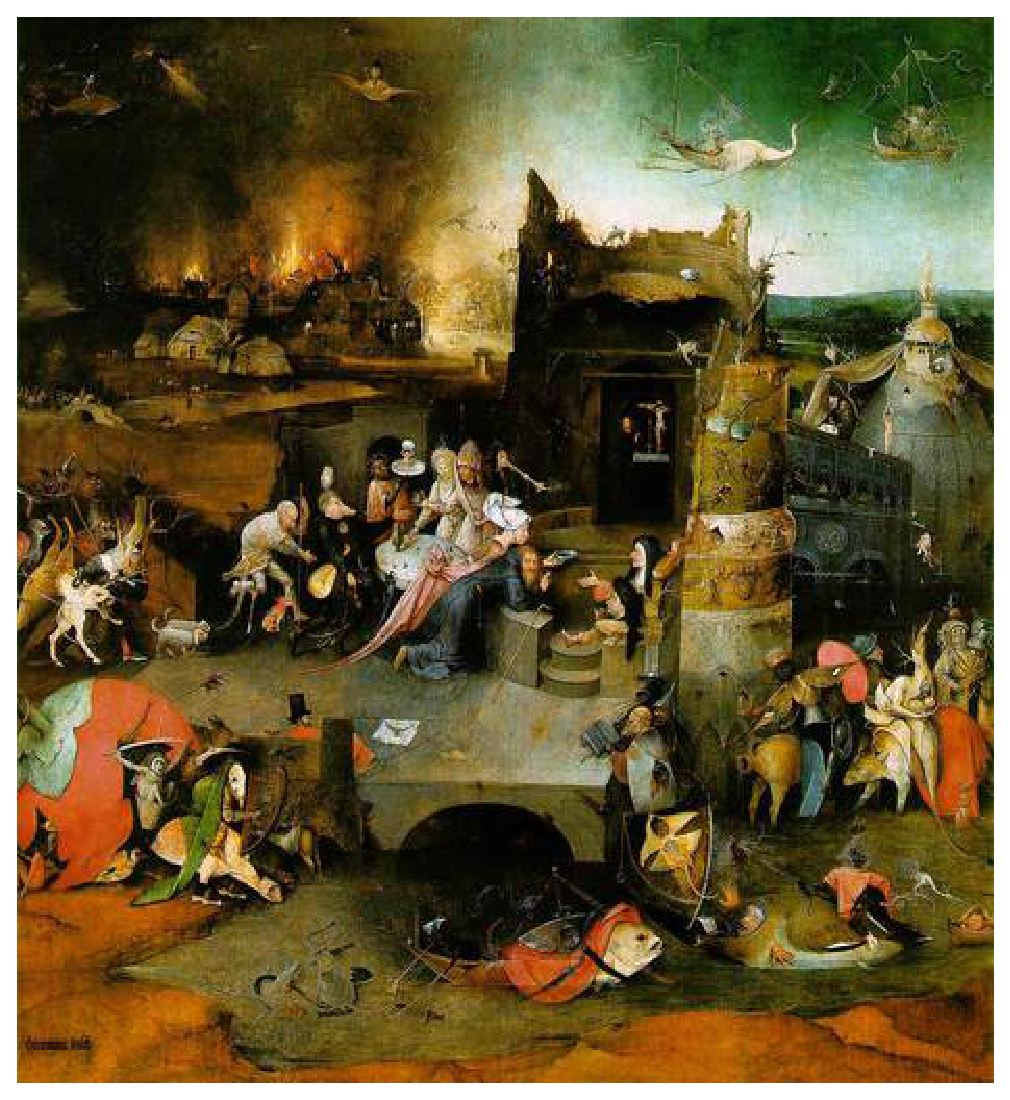
\includegraphics[width=0.25\linewidth]{original}
\label{fig:original}
}
\hspace{4ex}
\subfigure[]{
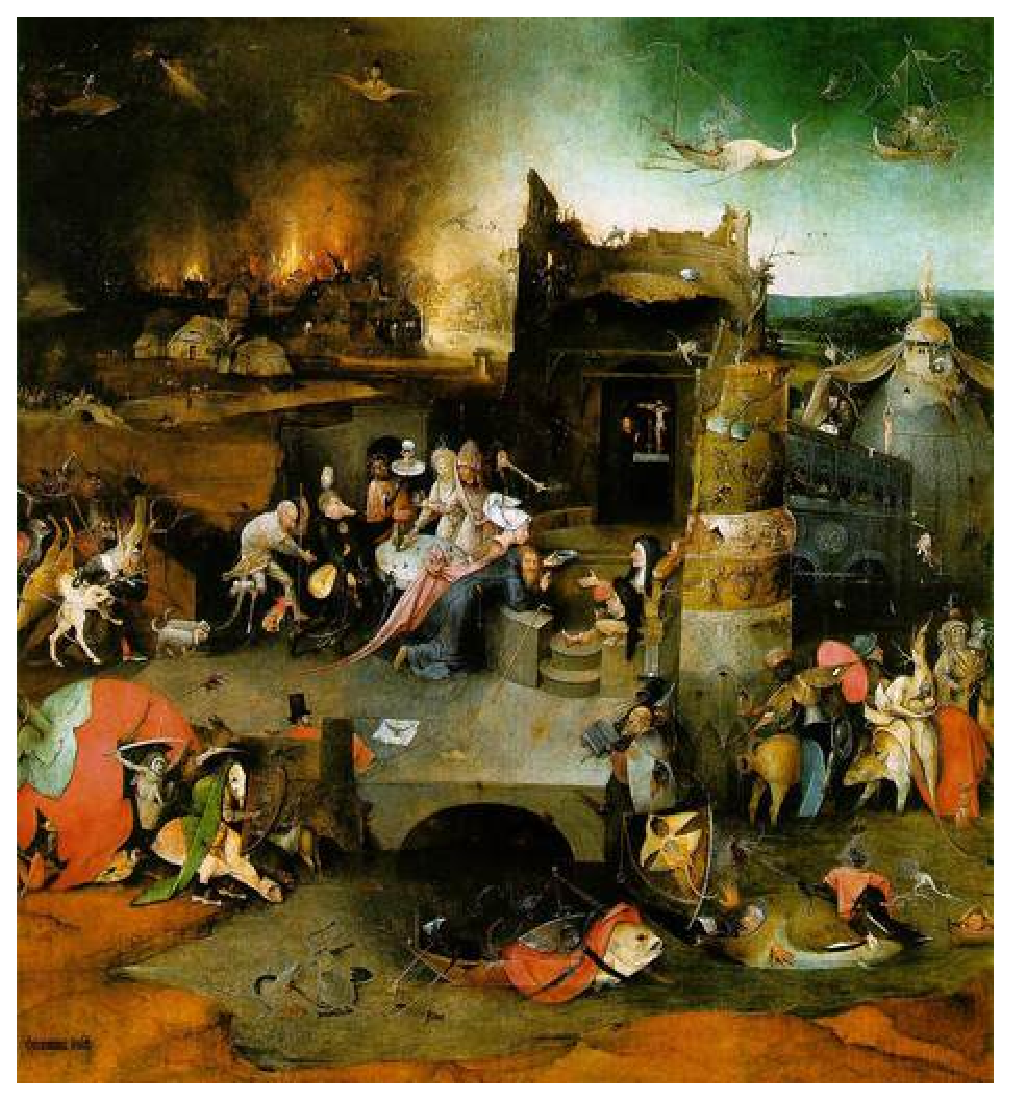
\includegraphics[width=0.25\linewidth]{steghide1}
\label{fig:steghide1}
}
\hspace{4ex}
\subfigure[]{
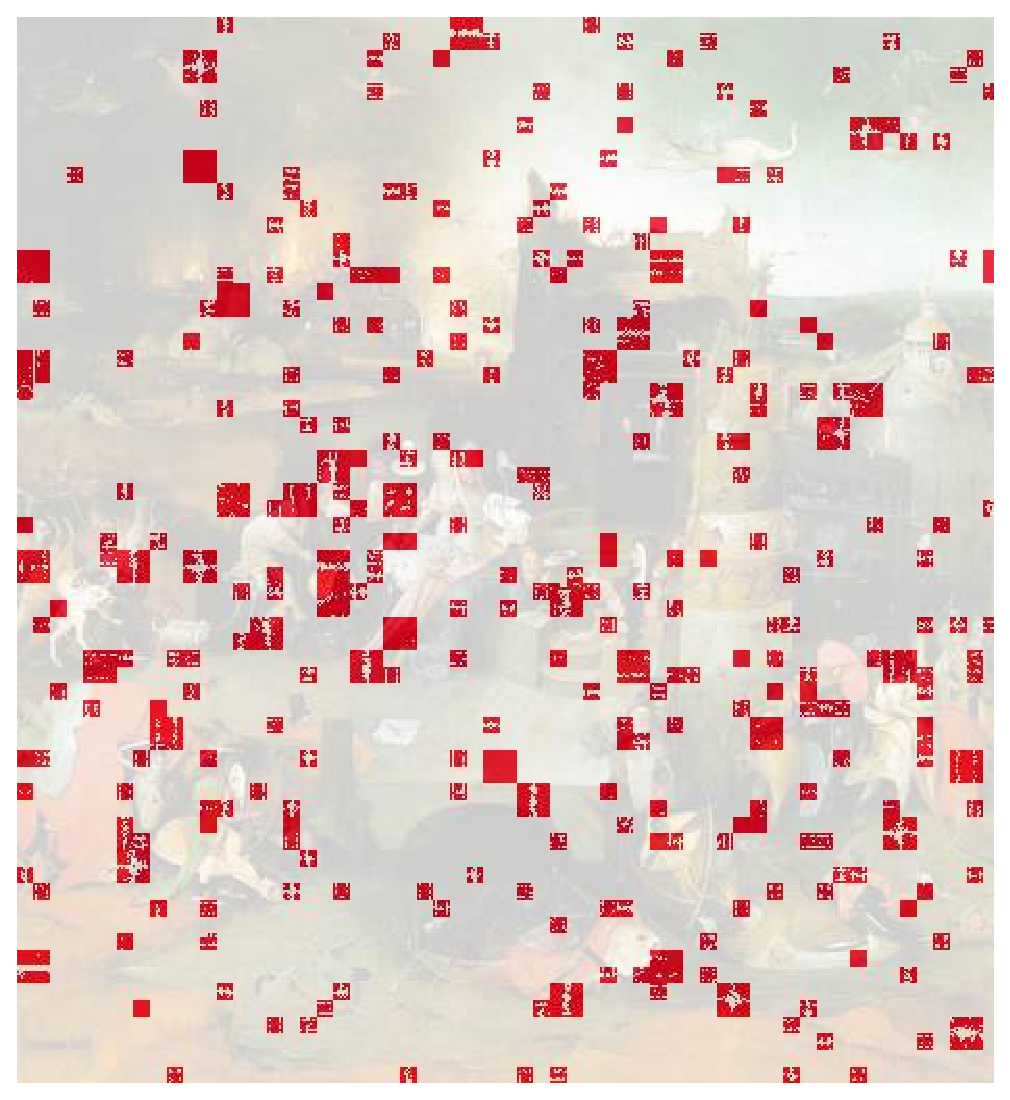
\includegraphics[width=0.25\linewidth]{steghide2}
\label{fig:steghide2}
}
\caption{Использование steghide: 
\subref{fig:original} исходное изображение; 
\subref{fig:steghide1} в изображении закодирована фраза <<Feci quod potui, faciant meliora potentes>> с паролем <<cogitoergosum>>; 
\subref{fig:steghide2}} разница между изображениями.
\end{figure}
Вставка данных в изображение:
\begin{lstlisting}
steghide embed -cf "coverfile.jpg" -ef "embedfile.txt" -sf "stegofile.jpg" -p "password"
\end{lstlisting}
coverfile.jpg --- файл, в который вставляются данные.\\
embedfile.txt --- файл, который вставляется в изображение.\\
stegofile.jpg --- файл со вставленным изображением.\\
password --- пароль.\\\\
Извлечение данных:
\begin{lstlisting}
steghide extract -sf "stegofile.jpg" -p "password" -xf "extractfile.txt"
\end{lstlisting}
stegofile.jpg --- файл со вставленным изображением.\\
password --- пароль.\\
extractfile.txt --- файл, в который нужно записать извлеченные данные.
\subsubsection{Недостатки}
\newpage %%%%% REMOVE LATER %%%%
\subsection{OpenStego}
\subsubsection{Установка}
Для установки посетите \url{http://openstego.sourceforge.net/} или установите пакет с помощью пакетного менеджера вашего дистрибутива.
\subsubsection{Использование}
\begin{figure}[h]
\center{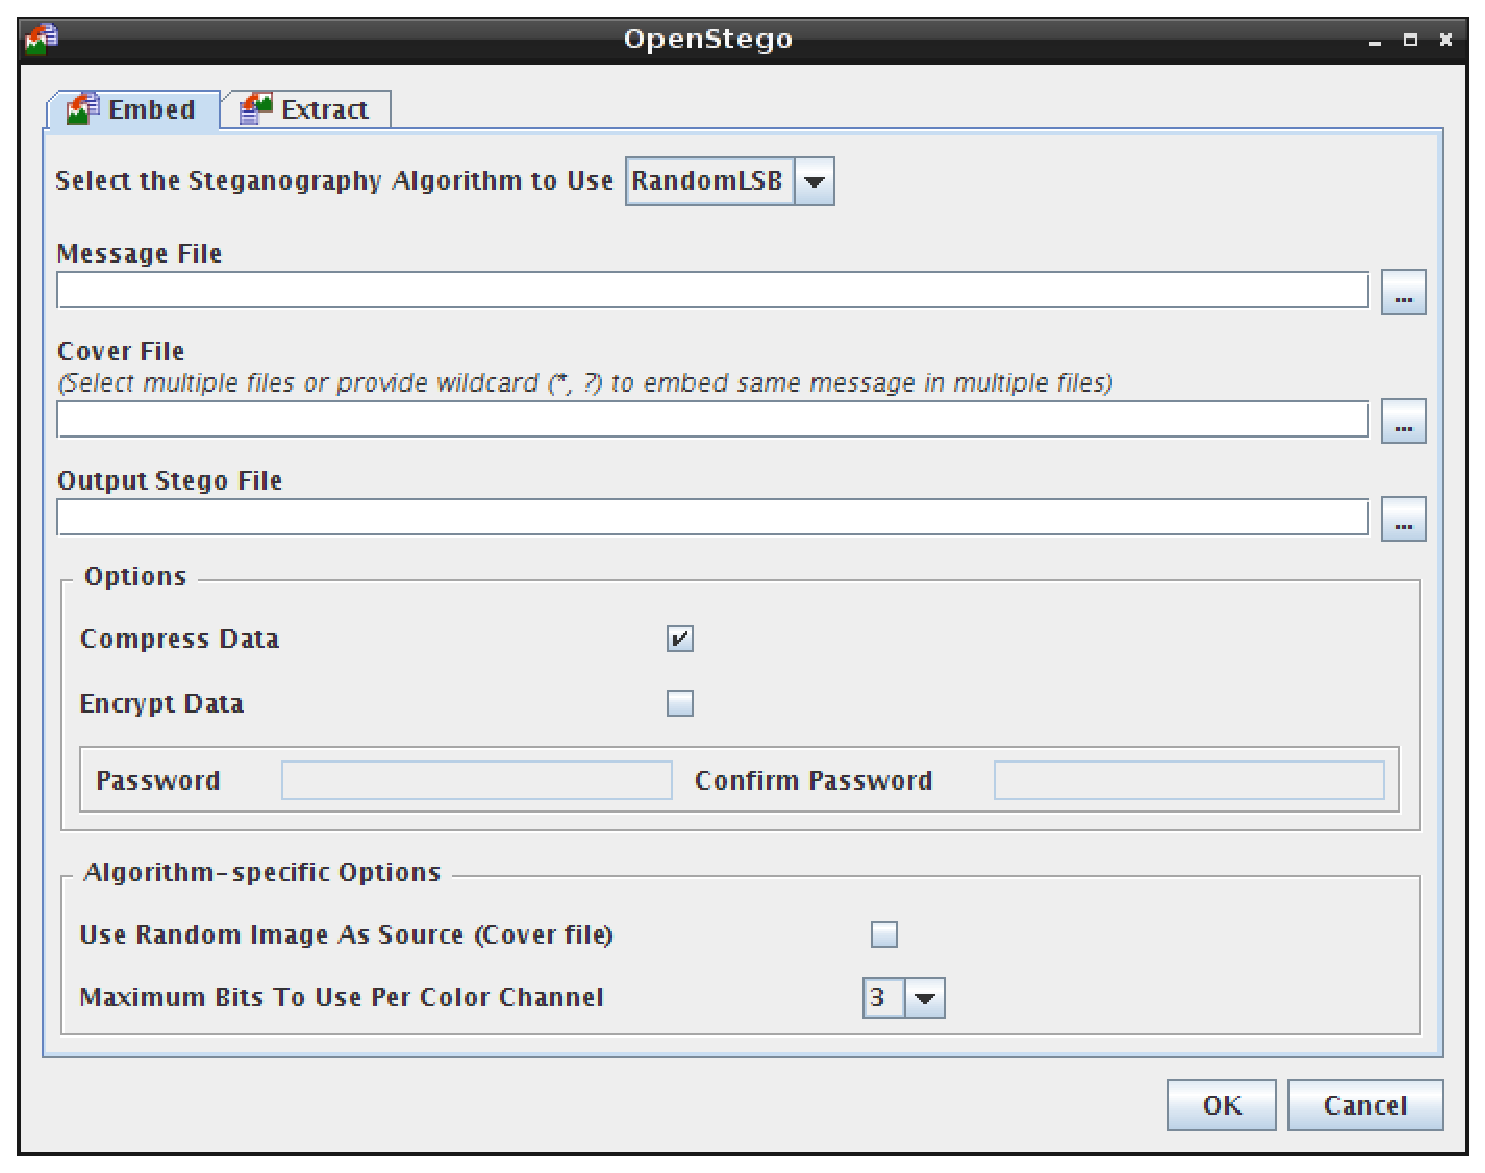
\includegraphics[width=0.75\linewidth]{openstego}}
\caption{Интерфейс OpenStego}
\end{figure}
\begin{figure}[ht!]
\vspace{-4ex}
\centering
\subfigure[]{
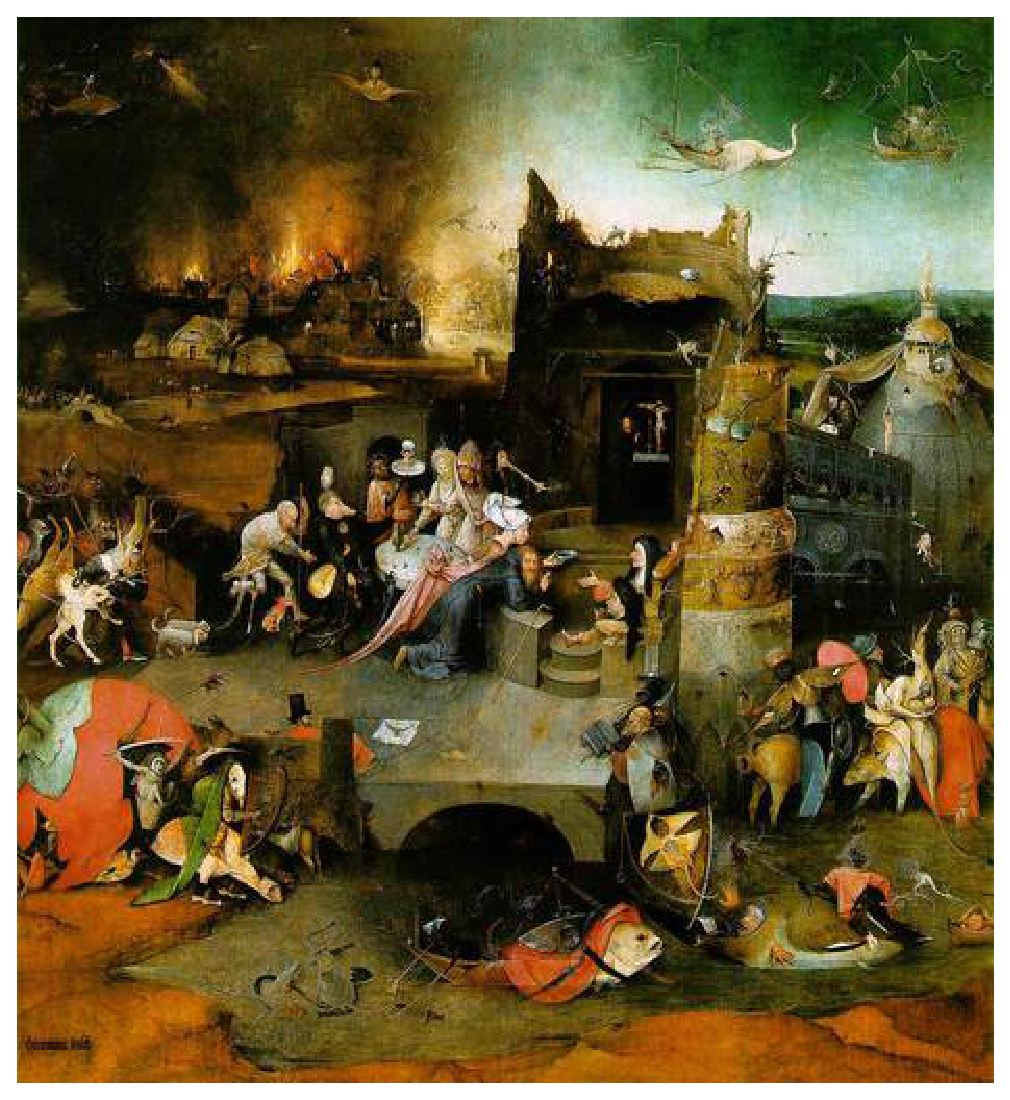
\includegraphics[width=0.25\linewidth]{original}
\label{fig:original}
}
\hspace{4ex}
\subfigure[]{
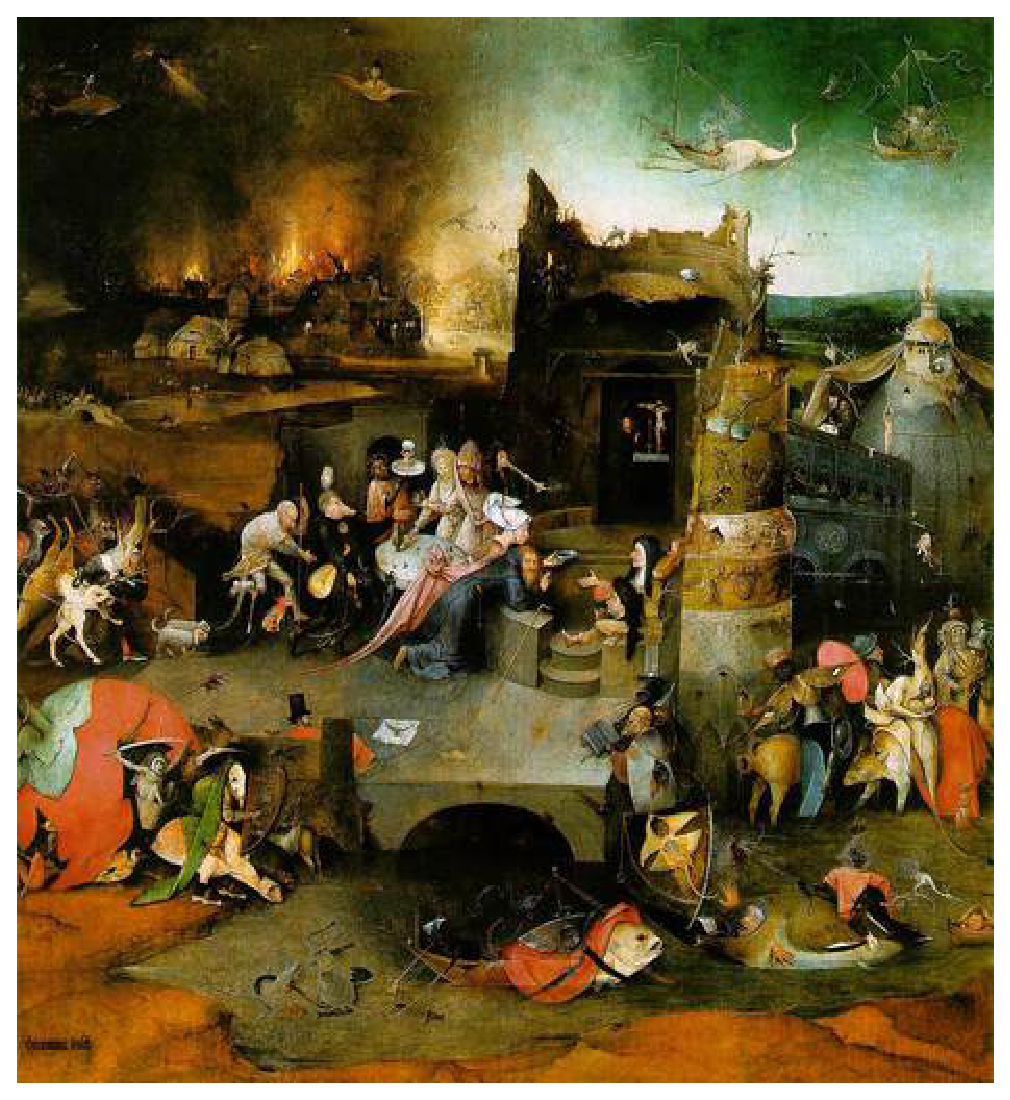
\includegraphics[width=0.25\linewidth]{openstego1}
\label{fig:openstego1}
}
\hspace{4ex}
\subfigure[]{

\includegraphics[width=0.25\linewidth]{openstego2}
\label{fig:openstego2}
}
\caption{Использование OpenStego:
\subref{fig:original} исходное изображение;
\subref{fig:openstego1} в изображении закодирована фраза <<Feci quod potui, faciant meliora potentes>> без пароля;
\subref{fig:openstego2}} разница между изображениями.
\end{figure}
\subsubsection{Недостатки}
\subsection{Желтые точки}
\begin{wrapfigure}[9]{r}{0.25\linewidth}
\includegraphics[width=\linewidth]{dots}
\caption{Желтые точки. Изображение: Parhamr}
\end{wrapfigure}
При печати материалов (например, листовок) не стоит забывать, что многие принтеры кодируют микроточками информацию о времени печати и о серийном номере принтера \cite{eff_dots}. Данная информация может быть использована для установления личности авторов отпечатков. Список принтеров, размещающих и не размещающих желтые точки смотрите в отчете Electronic Frontier Foundation\cite{eff_list}.

\section{Альтернативные DNS}
\subsection{Namecoin}
\subsection{OpenNIC}
\subsection{Собственный кеширующий DNS сервер}
